\section{Architecture} \label{sec:arch}

\xxx deployment is similar to a typical State Machine Replication (SMR) system: 
it runs a server program on replicas within a datacenter. Replicas connect with 
each other using RDMA QPs. Client programs are located in LAN or WAN.

\begin{figure*}[ht]
\begin{center}
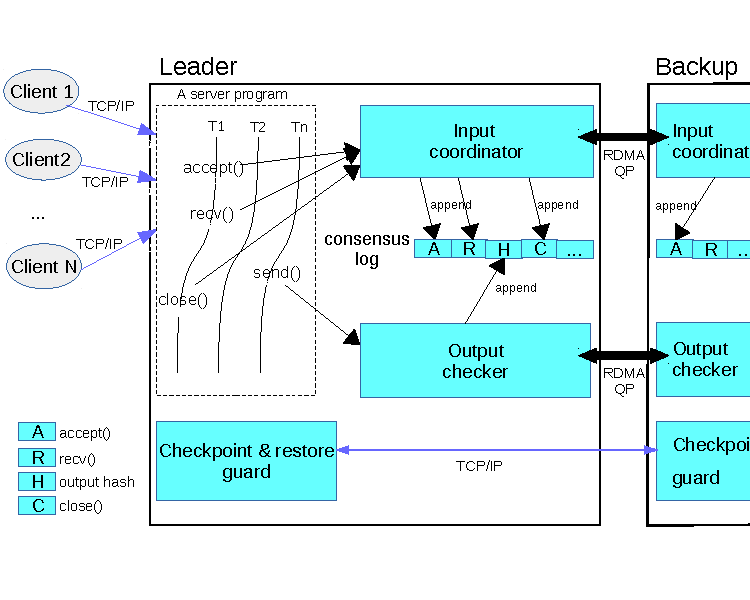
\includegraphics{figures/arch}
\caption{\em \xxx Architecture (key components are in
  blue).}\label{fig:arch}
\end{center}
\end{figure*}

The \xxx leader handles client requests and runs its RDMA-based protocol to 
enforce the same total order for all requests across replicas.

Figure~\ref{fig:arch} shows \xxx's architecture. \xxx intercepts a server 
program's inbound socket calls (\eg, \recv) using a Linux technique called 
\ldpreload. \xxx involves four key components: a \paxos consensus protocol for 
input coordination (in short, the \emph{coordinator}), a circular in-memory 
consensus log (the \emph{log}), a guard process that handles checkpointing 
and recovering a server's process and file system state (the 
\emph{guard}), and an optional output checking tool (the \emph{checker}).

The coordinator is involved when a thread of a program running on the \xxx 
leader calls an inbound socket call (\eg, \recv). The thread executes the 
Libc call, gets the received data, appends a log entry on the leader's local 
consensus log, and replicates this entry to backups' consensus logs using our 
\paxos protocol (\S\ref{sec:protocol}).

In this protocol, all threads in the server program running on the leader 
replica can concurrently invoke consensus on their log entries (requests), but 
\xxx enforces a total order for all entries in the leader's local consensus 
log. As a consensus request, each thread does an RDMA WRITE to replicate its 
log entry to the corresponding log entry position on all \xxx backups. Each 
\xxx backup polls from the latest unagreed entry on its local consensus log; 
if it agrees with the proposed log entry, it does an RDMA WRITE to write a 
consensus reply on the leader's corresponding entry.

To ensure \paxos safety~\cite{paxos:practical}, all \xxx backups agree on the 
entries proposed from the leader in a total order without allowing any entry 
gap. When a majority of replicas (including the leader) has written a consensus 
reply on the leader's local entry, this entry has reached a consensus. By doing 
so, \xxx consistently enforces the same consensus log for both the leader and
backups.

The output checker is periodically invoked as a program replicated in \xxx 
executes outbound socket calls (\eg, \send). For every 1.5KB (MTU size) of 
accumulated outputs per connection, the checker unions the previous hash with 
current outputs and computes a new CRC64 hash. For simplicity, the output 
checker uses \xxx's input consensus protocol (\S\ref{sec:protocol}) to compare 
hashes across replicas.
